\documentclass[runningheads]{llncs}
\usepackage[T1]{fontenc}
\usepackage{amsmath,amssymb}
\usepackage{graphicx}
\usepackage{booktabs}
\usepackage{array}
\usepackage{microtype}
\usepackage{tikz}

\renewcommand{\topfraction}{.9}\renewcommand{\bottomfraction}{.8}\renewcommand{\textfraction}{.08}\renewcommand{\floatpagefraction}{.75}
\usetikzlibrary{arrows.meta,positioning,fit,backgrounds}
\newcommand{\bfivezerothreeerrfivezerothreefixed}{2}
\newcommand{\bfivezerothreeerrfivezerothreelegacy}{160}
\newcommand{\bfivezerothreehealthyfixed}{40}
\newcommand{\bfivezerothreemederrfivezerothreefixed}{0.002}
\newcommand{\bfivezerothreemederrfivezerothreelegacy}{0.302}
\newcommand{\bfivezerothreemedhealthyfixed}{0.134}
\newcommand{\efivehangBnew}{24.72}
\newcommand{\efivehangBnewhttp}{80}
\newcommand{\efivehangBnewtot}{494.9}
\newcommand{\efivehangBold}{24.71}
\newcommand{\efivehangBoldhttp}{80}
\newcommand{\efivehangBoldtot}{494.7}
\newcommand{\efivehangSPonetwozeronew}{6.18}
\newcommand{\efivehangSPonetwozeronewhttp}{25}
\newcommand{\efivehangSPonetwozeronewtot}{154.7}
\newcommand{\efivehangSPonetwozeroold}{6.18}
\newcommand{\efivehangSPonetwozerooldhttp}{25}
\newcommand{\efivehangSPonetwozerooldtot}{154.6}
\newcommand{\efivehangSPthreezeronew}{3.09}
\newcommand{\efivehangSPthreezeronewhttp}{13}
\newcommand{\efivehangSPthreezeronewtot}{80.5}
\newcommand{\efivehangSPthreezeroold}{3.09}
\newcommand{\efivehangSPthreezerooldhttp}{13}
\newcommand{\efivehangSPthreezerooldtot}{80.4}
\newcommand{\efivehangSPsixzeronew}{6.20}
\newcommand{\efivehangSPsixzeronewhttp}{25}
\newcommand{\efivehangSPsixzeronewtot}{154.8}
\newcommand{\efivehangSPsixzeroold}{6.18}
\newcommand{\efivehangSPsixzerooldhttp}{25}
\newcommand{\efivehangSPsixzerooldtot}{154.5}
\newcommand{\efiveokSPsixzeronew}{0.14}
\newcommand{\efiveokSPsixzeronewhttp}{40}
\newcommand{\efiveokSPsixzeronewtot}{3.4}
\newcommand{\efiveokSPsixzeroold}{0.13}
\newcommand{\efiveokSPsixzerooldhttp}{40}
\newcommand{\efiveokSPsixzerooldtot}{2.9}
\newcommand{\efiverecoverSPsixzeronew}{0.19}
\newcommand{\efiverecoverSPsixzeronewhttp}{35}
\newcommand{\efiverecoverSPsixzeronewtot}{58.1}
\newcommand{\efiverecoverSPsixzeroold}{0.15}
\newcommand{\efiverecoverSPsixzerooldhttp}{35}
\newcommand{\efiverecoverSPsixzerooldtot}{57.5}
\newcommand{\efiverefuseSPsixzeronew}{0.18}
\newcommand{\efiverefuseSPsixzeronewhttp}{25}
\newcommand{\efiverefuseSPsixzeronewtot}{4.7}
\newcommand{\efiverefuseSPsixzeroold}{0.17}
\newcommand{\efiverefuseSPsixzerooldhttp}{25}
\newcommand{\efiverefuseSPsixzerooldtot}{4.3}
\newcommand{\phagrci}{[$-$0.284,$-$0.170]}
\newcommand{\phagrmean}{$-$0.226}
\newcommand{\phagrsame}{8}
\newcommand{\phchgci}{[$-$4.50,$-$0.24]}
\newcommand{\phchgmean}{$-$2.67}
\newcommand{\phchgsame}{7}
\newcommand{\phfuci}{[+0.00,+1.76]}
\newcommand{\phfumean}{+0.59}
\newcommand{\phfusame}{1}
\newcommand{\phrevci}{[$-$3.12,$-$0.27]}
\newcommand{\phrevmean}{$-$1.88}
\newcommand{\phrevsame}{7}
\newcommand{\predAone}{supported}
\newcommand{\predAonezero}{contradicted}
\newcommand{\predAtwo}{supported}
\newcommand{\predAthree}{supported}
\newcommand{\predAfour}{supported}
\newcommand{\predAfive}{supported}
\newcommand{\predAsix}{supported}
\newcommand{\predAseven}{supported}
\newcommand{\predAeight}{supported}
\newcommand{\predAnine}{contradicted}
\newcommand{\predBone}{supported}
\newcommand{\predBtwo}{supported}
\newcommand{\predBthree}{supported}
\newcommand{\predBfour}{supported}
\newcommand{\predBfive}{supported}
\newcommand{\predBsix}{contradicted}
\newcommand{\scRecEight}{928}
\newcommand{\scRecSeven}{312}
\newcommand{\scRemEight}{1{,}300}
\newcommand{\scSteady}{1{,}274}
\newcommand{\scStretch}{0}
\newcommand{\scTotal}{3{,}814}
\newcommand{\xaBzeroHigh}{2.056}
\newcommand{\xaBzeroMed}{0.546}
\newcommand{\xaMoneHigh}{4.411}
\newcommand{\xaMoneMed}{1.589}
\newcommand{\xaN}{160}
\newcommand{\xcsupported}{5}
\newcommand{\xctauzeroagr}{0.014}
\newcommand{\xctauzerochg}{2.225}
\newcommand{\xctaufiveagr}{0.400}
\newcommand{\xctaufivechg}{12.450}
\newcommand{\xctausixagr}{0.400}
\newcommand{\xctausixchg}{12.450}
\newcommand{\xctausevenagr}{0.400}
\newcommand{\xctausevenchg}{12.450}
\newcommand{\xctaueightagr}{0.404}
\newcommand{\xctaueightchg}{12.450}
\newcommand{\xctaunineagr}{0.626}
\newcommand{\xctauninechg}{15.119}
\newcommand{\xdOverlap}{17}
\newcommand{\xdPlaceholder}{64}
\newcommand{\xeEoneDiff}{0}
\newcommand{\xeEoneIdentical}{yes}
\newcommand{\xeEoneRows}{752}

\emergencystretch=2em
\begin{document}

\title{Specialization and Coordination in a Multi-Agent Technical Interview System: Trajectory Dynamics and Architectural Trade-offs}
\titlerunning{Specialization and Coordination in a Multi-Agent Interview System}
\author{Anonymous Author(s)}
\authorrunning{Anonymous}
\institute{Anonymous Institution}
\maketitle

\begin{abstract}
Educational and conversational systems that combine automated evaluation, language models, and reinforcement-learning controllers are frequently labelled multi-agent, even when a single monolithic controller invokes components procedurally. We investigate whether decomposing pedagogical decision-making into specialized, stateful agents with a coordination layer yields measurable behavioral, trajectory, or decision-making advantages over a single-controller baseline. We extend an orchestrated technical-interview preparation system with two bounded-authority agents: a Strategy Agent managing a persistent weakness ledger across turns (proposing difficulty transitions and follow-up probes) and a Coaching Agent managing a coaching history ledger (proposing feedback depth, hints, and instructional emphasis), coordinated via unidirectional peer messaging and threshold-gated arbitration. Evaluating across 160 deterministic replay sessions (8 recorded candidate answer clusters across 20 question orders; no live language model ran), we find that stateful coordination alters difficulty trajectories in all 160 sessions relative to the frozen single-policy PPO baseline, smoothing level changes ($15.12 \to 12.45$; cluster-bootstrap 95\% CI $[-4.50, -0.24]$) and reversals ($11.74 \to 9.87$; cluster CI $[-3.12, -0.27]$), while reducing PPO agreement ($1.000 \to 0.774$) and introducing $+0.59$ probe turns driven specifically by one answer cluster ($k=1$). However, our findings challenge the assumption that agent specialization inherently optimizes decision quality: an ablated coaching configuration and an equivalent unified agent produce mathematically identical difficulty trajectories ($\mathbb{P}(\text{agree}) = 1.0$). The value of specialization lies not in algorithmic decision superiority, but in software modularity, independent state auditability, and bulkhead fault containment, balanced against $+1.04$\,ms median per-turn dispatch overhead. Threshold sensitivity experiments ($\tau \in [0.0, 0.9]$) isolate the confidence threshold as the critical gating mechanism preventing oscillation collapse. We make no claims of human candidate learning or live model performance.
\keywords{multi-agent coordination \and agent specialization \and decision-making \and trajectory dynamics \and interview practice \and arbitration}
\end{abstract}

\section{Introduction}\label{sec:intro}
Interactive educational systems that combine automated scoring, language models, and reinforcement-learning (RL) policies are increasingly described as multi-agent systems~\cite{autogen,metagpt}, even when a single monolithic controller executes every component in a fixed procedural pipeline. Whether the multi-agent label reflects a genuine scientific distinction depends on how authority and state are distributed~\cite{wj95}. If components operate as specialized autonomous agents, critical questions arise regarding coordination, decision consistency, and architectural necessity: how do specialized agents coordinate their recommendations, how does their interaction affect session trajectories, and does partitioning responsibilities across specialized agents provide measurable value over a unified controller?

We investigate these questions within an orchestrated spoken technical-interview preparation system whose production architecture we audit rather than assume. In its baseline configuration, the system executes an automated interview workflow driven by a single learned policy (a frozen Proximal Policy Optimization controller~\cite{ppo,sb3}) operating over a 6-dimensional state vector without concept memory. Every other pedagogical choice is governed by static threshold rules in the central hub. We extend this system by introducing two specialized, stateful agents behind a feature flag, leaving the underlying evaluator, frozen PPO policy, and candidate contract intact:
\begin{enumerate}
\item \textbf{Strategy Agent:} Maintains a private weakness ledger across turns, tracking persistent conceptual deficiencies and score trajectories to propose dynamic difficulty transitions and proactive follow-up probes.
\item \textbf{Coaching Agent:} Maintains a private coaching history ledger, tracking previously delivered hints and examples to propose feedback depth, instructional emphasis, and targeted remediation tags.
\end{enumerate}
The agents possess strictly bounded authority: they only \emph{propose}. A deterministic coordinator validates all proposals against formal schemas and authority matrices, an arbitrator resolves competing recommendations against safety bounds and the PPO policy, and the central hub remains the sole system of record. Crucially, the Strategy Agent communicates pedagogical intent to the Coaching Agent via unidirectional peer messaging, enabling aligned instructional guidance without coupling private state ledgers.

This architecture enables a rigorous empirical evaluation of multi-agent coordination and specialization. Rather than evaluating generic agent reliability or treating multi-agent design as an axiomatic virtue, we formulate three precise research questions:
\begin{description}
\item[RQ1 (Coordination and intervention dynamics):] How does stateful coordination between the Strategy and Coaching agents affect the decisions and session trajectories of the interview preparation system, compared with the frozen single-policy baseline ($B_0$)?
\item[RQ2 (Value of agent specialization):] Does separating Strategy and Coaching into distinct specialized agents provide measurable benefits over a unified technical coaching agent operating on equivalent information and tasks?
\item[RQ3 (Coordination mechanisms):] Which implemented coordination components---stateful memory, peer messaging, confidence threshold gating, or PPO interaction---are responsible for observable differences in system decisions?
\end{description}

\noindent\textbf{Summary of Findings and Contributions.}
\begin{itemize}
\item \emph{Coordination Dynamics (RQ1):} In deterministic replay across 160 sessions (evaluating 64 recorded human-interview evaluator payloads across 20 question orders), stateful coordination alters difficulty trajectories in all 160 sessions relative to the frozen baseline. The Strategy Agent smooths trajectory oscillations, reducing mean level changes from 15.12 to 12.45 per session ($-2.67$, cluster-bootstrap 95\% CI \phchgci{}) and mean reversals from 11.74 to 9.87 ($-1.88$, cluster CI \phrevci{}). Agreement with the uncoordinated PPO action decreases from 1.000 to 0.774 ($-0.226$, cluster CI \phagrci{}). Proactive probes introduce an average of $+0.59$ additional turns per session (cluster CI \phfuci{}). However, a cluster sensitivity analysis reveals that this probing increase is driven entirely by a single recorded answer cluster ($k=1$); omitting cluster 1 yields $\Delta = +0.00$ extra turns.
\item \emph{Limits of Specialization (RQ2):} We demonstrate that under deterministic decision rules, agent specialization yields \textbf{zero algorithmic or trajectory advantage}. Ablating the Coaching Agent ($M_3$) reproduces the full two-agent system's difficulty trajectory in 160 of 160 sessions, and a unified agent operating on equivalent state produces mathematically identical decisions ($\mathbb{P}(\text{agree}) = 1.0$). Specialization introduces a measurable dispatch overhead ($+1.04$\,ms median per turn; 47.7 agent calls per session). The defensible benefits of specialization are strictly software-engineering properties: disjoint state ledgers, independent unit testing, and isolated failure containment.
\item \emph{Mechanism Decomposition (RQ3):} Through controlled ablations and a multi-level threshold sweep ($\tau \in [0.0, 0.9]$), we isolate the confidence threshold as the critical gating mechanism. Setting $\tau = 0.0$ collapses level changes to 2.225 and PPO agreement to 0.014, identical to removing arbitration entirely ($M_4$). Peer messaging ($M_5$) alters coaching depth and tone without destabilizing difficulty. Disabling PPO ($M_7$) alters trajectories in only 4 of 160 sessions (2.5\%), contradicting the registered prediction of $\ge 50\%$ divergence and revealing strong alignment between the Strategy Agent heuristic and the baseline rule fallback.
\end{itemize}

\noindent\textbf{What Kind of Contribution This Is.} The specialized agents, typed contracts, and authority matrix constitute \emph{architecture}; the peer messaging and threshold gating constitute \emph{coordination mechanisms}; the replay ablations and cluster-bootstrap evaluations provide \emph{empirical evidence on coordination and the limits of specialization}.

\noindent\textbf{Explicit Disclaimers.} All replay experiments execute deterministically with recorded evaluator outputs (`EVALUATOR\_MOCK\_MODE=1`); no live large language model was invoked during replay. We make \textbf{no claims} regarding candidate learning, pedagogical efficacy, interview placement success, or LLM hallucination rates. Fewer trajectory reversals reflect behavioral stability, not proven pedagogical superiority.

\section{Related Work}\label{sec:related}
\noindent\textbf{Multi-Agent Coordination and Specialization.} The classic characterization of agency by Wooldridge and Jennings defines agents through autonomy, reactivity, pro-activeness, and social ability~\cite{wj95}. In modern LLM-based systems, multi-agent frameworks predominantly follow two coordination paradigms: conversational emergent interaction, exemplified by AutoGen~\cite{autogen}, and structured role-based workflows with standardized operating procedures, exemplified by MetaGPT~\cite{metagpt}. While these frameworks demonstrate qualitative versatility across software development and debate tasks, recent empirical audits demonstrate that multi-agent LLM systems frequently suffer from coordination collapse, specification drift, and inter-agent misalignment~\cite{mast,resil,masfire}. Crucially, literature often assumes that decomposing a complex task into multiple specialized agents is inherently advantageous. However, few studies isolate whether specialization provides measurable decision-making benefits over a unified controller operating with equivalent information. Our work directly evaluates this trade-off by comparing specialized stateful agents against an uncoordinated baseline and an equivalent unified architecture.

\noindent\textbf{Adaptive Mock Interview and Tutoring Systems.} AI-assisted interview systems have emerged to provide automated feedback and dynamic evaluation for technical candidates. Systems such as Zara~\cite{zara} utilize generative LLMs to synthesize candidate feedback, while empirical user studies investigate student confidence, readiness, and trust in automated code evaluation~\cite{virt,chase}. However, generative LLMs often exhibit verbosity, position bias, and hallucinations when tasked with simultaneous scoring and pedagogical planning~\cite{judge}. To ensure evaluation integrity, our target system enforces strict authority boundaries derived from the principle of least privilege~\cite{ss75}: scoring is computed by a deterministic, cross-encoder evaluator outside the language model, while agents operate solely on validated observations.

\noindent\textbf{Reinforcement Learning, Shielding, and Coordination Envelopes.} Dynamic difficulty adaptation in educational platforms is commonly framed as a reinforcement learning problem. Single-agent RL approaches, such as Proximal Policy Optimization (PPO)~\cite{ppo} implemented via Stable-Baselines3~\cite{sb3}, optimize policy returns over state trajectories. However, unconstrained RL policies risk erratic behavior during out-of-distribution candidate interactions. Safe reinforcement learning surveys~\cite{safe} classify external knowledge mechanisms, such as shielding~\cite{shield}, as essential safety envelopes that override learned actions when constraints are violated. Our arbitration architecture implements an empirical safety envelope where rule-based, evidenced agent proposals compete with the frozen PPO action while remaining bounded by deterministic guardrails. This architecture represents centrally orchestrated role specialization rather than Multi-Agent Reinforcement Learning (MARL)~\cite{marl}, as the PPO policy is frozen and the agents do not update policy weights dynamically.

\noindent\textbf{Methodological Foundations and Dependability.} To evaluate coordination integrity, we draw upon dependable computing taxonomies~\cite{alrl04}, enforcing bulkhead isolation via per-agent circuit breakers~\cite{nygard} to bound cascading failures. For statistical inference over replayed candidate answer clusters, we employ clustered bootstrapping methodologies established by Field and Welsh~\cite{fw07}, preventing artificially narrow confidence intervals that arise from treating permuted question sequences as independent candidate samples.

\section{The Existing System and What Was Added}\label{sec:design}
\subsection{Existing workflow (preserved)}
A browser client sends a spoken answer to a backend, which transcribes it and calls an \emph{InterviewOrchestrator} (the hub). The hub owns one session-state dictionary and one lock and runs a fixed per-turn pipeline: (1) a learned \emph{evaluator} (sentence-embedding similarity, a concept index and a fine-tuned cross-encoder; $0.15S_1{+}0.35S_2^{\mathrm{eff}}{+}0.50R$ with a cap when a mandatory concept is missed) returns a score and concept evidence; (2) a strict hand-off contract treats a non-finite or out-of-range score as an evaluator failure and fails closed; (3) feedback is produced by a template or an optional local LLM; (4) the hub commits the turn; (5) a baseline schedule and then a frozen PPO policy~\cite{ppo,sb3} propose an easier/same/harder action, followed by a rule layer of six guardrails; (6) a threshold rule decides whether a follow-up question is injected (at most two in a row). Before this work only the PPO policy was a reactive learned decision-maker; the LLM never chose an action. All of this is unchanged when the multi-agent flag is off, and a test shows that with the flag on but no agent contributing the trajectory is identical (Sect.~\ref{sec:results}).

\subsection{Agents}
\begin{table}[tbp]
\centering\small
\caption{Authority matrix, generated from the enforcing code (\texttt{agents/multiagent/} \texttt{authority.py}). Neither agent has state-write authority; the hub commits alone.}\label{tab:authority}
\begin{tabular}{>{\raggedright\arraybackslash}p{1.5cm}>{\raggedright\arraybackslash}p{2.5cm}>{\raggedright\arraybackslash}p{2.3cm}>{\raggedright\arraybackslash}p{2.8cm}>{\raggedright\arraybackslash}p{2.0cm}}
\toprule
Agent & May propose & Private state & Cannot & On invalid output \\
\midrule
\textbf{Strategy} & difficulty\_action (Easier/Same/Harder); probe request (concept, kind); strategy mode & weakness ledger (per-concept miss counts, probe history, trend) & write or overwrite any score; set a difficulty level directly; terminate the session; edit history; override hard constraints or guardrail overrides; call another agent & invalid / stale / low-confidence / timed-out proposal is dropped; PPO proposal stands \\
\midrule
\textbf{Coaching} & feedback depth; hint / example flags; concepts to emphasise; remediation tag; tone & coaching history (hints/examples given, repeated misconceptions) & alter evaluator results or scores; cite concepts absent from the evaluator evidence; request difficulty changes; request follow-ups; terminate the session & invalid plan is dropped; the existing template feedback is used unchanged \\
\bottomrule
\end{tabular}

\end{table}
Table~\ref{tab:authority} lists what each agent may propose and may not do. Applying the principle of least privilege~\cite{ss75}, neither agent possesses state-write privileges. Both agents implement a single method \texttt{propose(observation, peer)}, receive an immutable, validated \texttt{TurnObservation} (score, evidence lists, difficulty, score history, progress, follow-up counters; counters carry the value the hub will commit), and return a typed proposal. They are rule- and ledger-based, not LLM-driven; they are the smallest design that has private persistent state, pro-active proposals and a communication channel, which are the properties of weak agency~\cite{wj95} that the existing roles lacked. We make no claim of autonomy beyond that.

\paragraph{Strategy Agent.} Objective: keep the candidate in productive difficulty while resolving persistent weaknesses within the follow-up budget. Private state: per concept, the distinct turns in which the evaluator listed it as missing or incorrect, which concepts were later covered, probes already requested, and an exponential moving average of scores. Rules, first match wins: \emph{recover} (current score $<0.35$ and mean of the last two $<0.5$, or a weakness that survived its probes while the score stays $<0.5$) $\rightarrow$ Easier; \emph{remediate} (a concept missed on $\ge 2$ distinct turns and unresolved) $\rightarrow$ Same plus a probe request for that concept; \emph{stretch} (score $\ge0.8$, average $\ge0.7$, last three $\ge0.6$, no open weakness) $\rightarrow$ Harder; otherwise \emph{steady}. Confidence is $\min(0.95, 0.5{+}0.1n)$ for $n$ cited evidence items, a documented heuristic and not a calibrated probability; the score itself is always one cited item, so a non-\emph{steady} proposal cites two or three items and carries 0.70 or 0.80; \emph{steady} proposals carry 0.45, below the arbitration threshold $\tau{=}0.6$, so the PPO action stands unless the ledger supports a change.

\paragraph{Coaching Agent.} Objective: choose how to coach after an evaluated answer. Private state: concept miss counts and the hints and examples already given. Decisions: up to two concepts to emphasise (incorrect claims first, then repeatedly missed, then evaluator order); a hint if concepts are missing, the score is $<0.6$ and fewer than two hints were given for the lead concept; an example when the lead concept was missed before and no example was given yet; depth (\emph{detailed} if score $<0.4$ or a repeated miss, \emph{brief} if $\ge0.85$ with nothing missing); tone; a remediation tag. A Strategy proposal delivered as a peer message modifies the plan (\emph{recover}: detailed and encouraging; \emph{stretch}: brief; \emph{remediate}: remediation tag on the probed concept). A deterministic renderer applies the plan to the existing feedback dictionary: it adds presentation fields and may prepend a priority tip to, or truncate, the existing improvement and communication-tip lists, and it raises if any protected evaluator field (score, grade, concept and claim lists, transcript, decision source) would change.

\subsection{Communication and state ownership}\label{sec:comm}
Every observation, proposal and decision is a typed object (\texttt{pydantic}, unknown fields rejected, NaN and out-of-range values rejected). The coordinator records each call as an envelope with session, turn, sender, recipient, state version and provenance, and every accept/reject/modify outcome as a decision record with a reason code. Optimistic concurrency uses a \emph{state version} that counts committed turns: a proposal whose version, turn or session differs from the observation, or from the hub's current version, is stale and dropped; a second answer from the same agent for the same version is a duplicate and dropped. The hub builds observations, commits state, increments the version, and persists agent memory in its session snapshot so that a recovered session resumes with the agents' ledgers.

\begin{figure}[tbp]
\centering
\resizebox{\textwidth}{!}{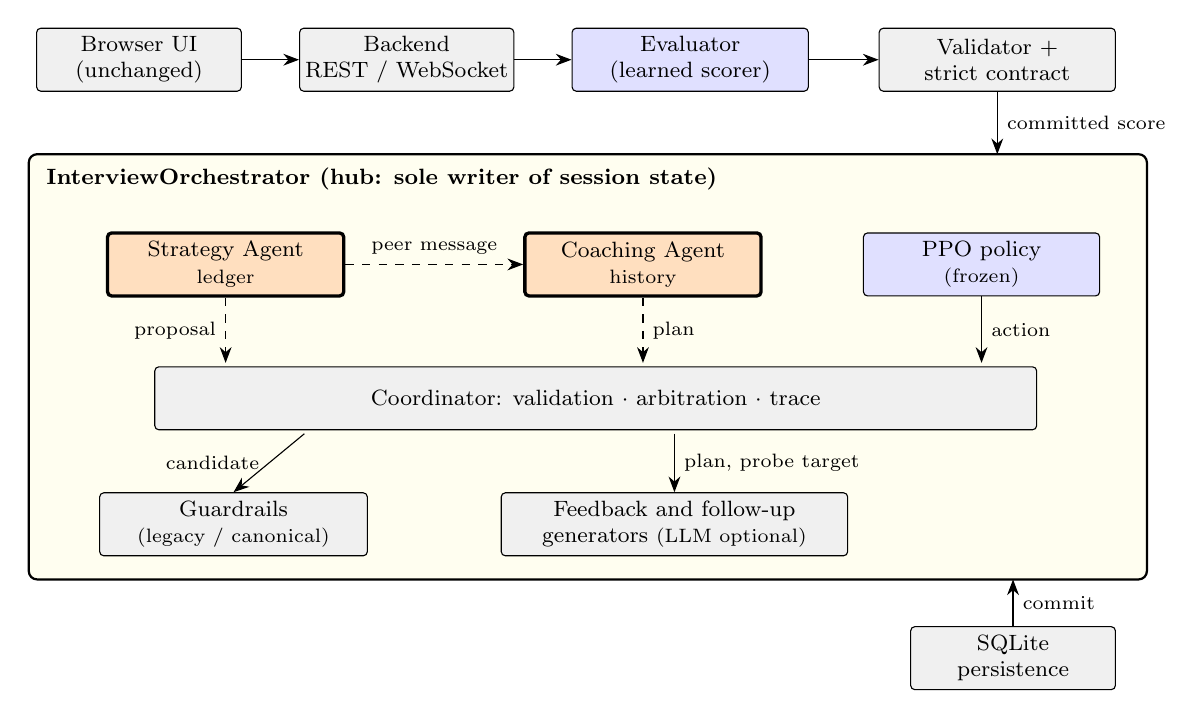
\begin{tikzpicture}[font=\footnotesize,
  box/.style={draw, rounded corners=1.5pt, minimum height=8mm, align=center, inner sep=2pt},
  det/.style={box, fill=gray!12},
  lrn/.style={box, fill=blue!12},
  agt/.style={box, fill=orange!25, very thick},
  arr/.style={-{Stealth[length=2mm]}, thin},
  darr/.style={-{Stealth[length=2mm]}, thin, dashed}]
% outside the hub
\node[det, minimum width=26mm] (ui) at (0.5,6.2) {Browser UI\\(unchanged)};
\node[det, minimum width=26mm] (be) at (3.9,6.2) {Backend\\REST / WebSocket};
\node[lrn, minimum width=30mm] (ev) at (7.5,6.2) {Evaluator\\(learned scorer)};
\node[det, minimum width=30mm] (val) at (11.4,6.2) {Validator +\\strict contract};
\draw[arr] (ui) -- (be); \draw[arr] (be) -- (ev); \draw[arr] (ev) -- (val);
% hub
\draw[rounded corners=3pt, thick, fill=yellow!6] (-0.9,-0.4) rectangle (13.3,5.0);
\node[anchor=north west, font=\footnotesize\bfseries] at (-0.8,4.95) {InterviewOrchestrator (hub: sole writer of session state)};
\node[agt, minimum width=30mm] (st) at (1.6,3.6) {Strategy Agent\\{\scriptsize ledger}};
\node[agt, minimum width=30mm] (co) at (6.9,3.6) {Coaching Agent\\{\scriptsize history}};
\node[lrn, minimum width=30mm] (pp) at (11.2,3.6) {PPO policy\\{\scriptsize (frozen)}};
\node[det, minimum width=112mm] (cd) at (6.3,1.9) {Coordinator: validation $\cdot$ arbitration $\cdot$ trace};
\node[det, minimum width=34mm] (gr) at (1.7,0.3) {Guardrails\\{\scriptsize (legacy / canonical)}};
\node[det, minimum width=44mm] (fb) at (7.3,0.3) {Feedback and follow-up\\generators {\scriptsize (LLM optional)}};
\node[det, minimum width=26mm] (db) at (11.6,-1.4) {SQLite\\persistence};
\draw[arr] (val.south) -- node[right]{\scriptsize committed score} (11.4,5.0);
\draw[darr] (st) -- node[above]{\scriptsize peer message} (co);
\draw[darr] (st.south) -- node[left]{\scriptsize proposal} (1.6,2.35);
\draw[darr] (co.south) -- node[right]{\scriptsize plan} (6.9,2.35);
\draw[arr] (pp.south) -- node[right]{\scriptsize action} (11.2,2.35);
\draw[arr] (2.6,1.45) -- node[left]{\scriptsize candidate} (gr.north);
\draw[arr] (7.3,1.45) -- node[right]{\scriptsize plan, probe target} (fb.north);
\draw[arr] (db.north) -- node[right]{\scriptsize commit} (11.6,-0.4);
\end{tikzpicture}
}
\caption{Implemented architecture. Shaded orange: the two added agents; blue: learned components; grey: deterministic infrastructure. Dashed arrows are typed proposals; agents never write state.}\label{fig:arch}
\end{figure}

\section{Orchestration, Arbitration and Validation}\label{sec:arbitration}
\begin{figure}[tbp]
\centering
\resizebox{0.97\textwidth}{!}{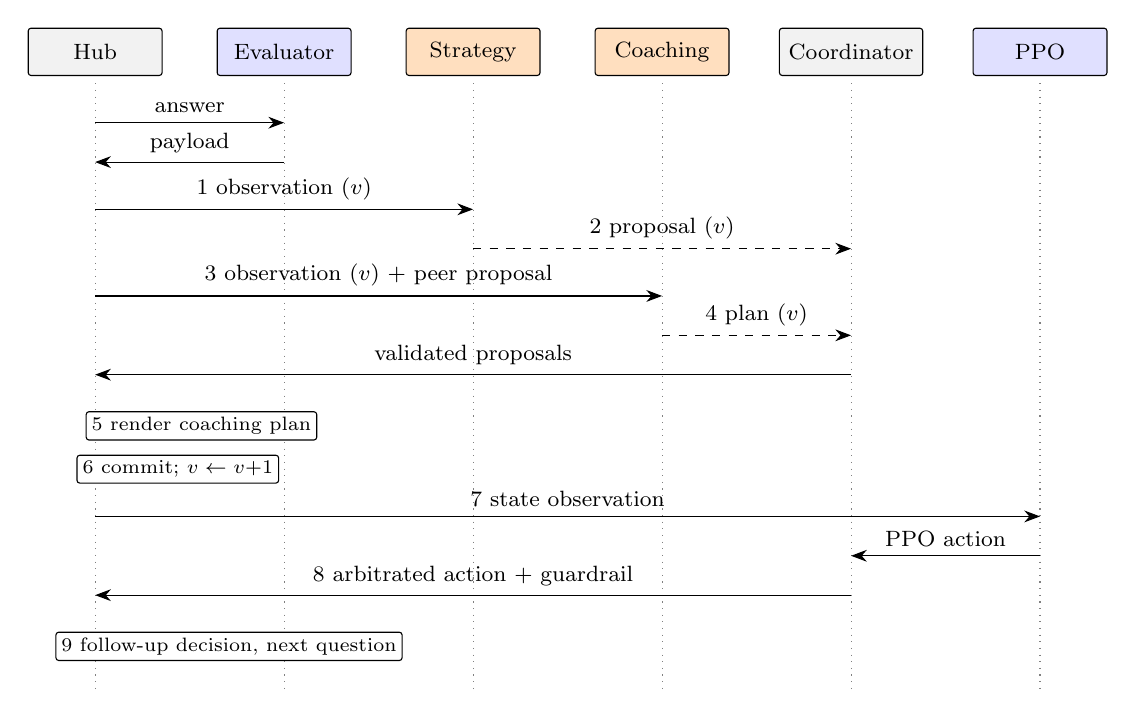
\begin{tikzpicture}[font=\footnotesize, x=1cm, y=1cm,
  life/.style={draw, rounded corners=1pt, minimum width=17mm, minimum height=6mm, align=center, fill=gray!10},
  msg/.style={-{Stealth[length=2mm]}, thin},
  dmsg/.style={-{Stealth[length=2mm]}, thin, dashed},
  note/.style={draw, fill=white, rounded corners=1pt, inner sep=2pt, font=\scriptsize}]
\def\xh{0} \def\xe{2.4} \def\xs{4.8} \def\xc{7.2} \def\xd{9.6} \def\xp{12}
\node[life] (hub) at (\xh,0) {Hub};
\node[life, fill=blue!12] (ev) at (\xe,0) {Evaluator};
\node[life, fill=orange!25] (st) at (\xs,0) {Strategy};
\node[life, fill=orange!25] (co) at (\xc,0) {Coaching};
\node[life] (cd) at (\xd,0) {Coordinator};
\node[life, fill=blue!12] (pp) at (\xp,0) {PPO};
\foreach \x in {\xh,\xe,\xs,\xc,\xd,\xp} \draw[gray, dotted] (\x,-0.4) -- (\x,-8.1);
\draw[msg] (\xh,-0.9) -- node[above]{answer} (\xe,-0.9);
\draw[msg] (\xe,-1.4) -- node[above]{payload} (\xh,-1.4);
\draw[msg] (\xh,-2.0) -- node[above]{1 observation $(v)$} (\xs,-2.0);
\draw[dmsg] (\xs,-2.5) -- node[above]{2 proposal $(v)$} (\xd,-2.5);
\draw[msg] (\xh,-3.1) -- node[above]{3 observation $(v)$ + peer proposal} (\xc,-3.1);
\draw[dmsg] (\xc,-3.6) -- node[above]{4 plan $(v)$} (\xd,-3.6);
\draw[msg] (\xd,-4.1) -- node[above]{validated proposals} (\xh,-4.1);
\node[note] at (\xh+1.35,-4.75) {5 render coaching plan};
\node[note] at (\xh+1.05,-5.3) {6 commit; $v \leftarrow v{+}1$};
\draw[msg] (\xh,-5.9) -- node[above]{7 state observation} (\xp,-5.9);
\draw[msg] (\xp,-6.4) -- node[above]{PPO action} (\xd,-6.4);
\draw[msg] (\xd,-6.9) -- node[above]{8 arbitrated action + guardrail} (\xh,-6.9);
\node[note] at (\xh+1.7,-7.55) {9 follow-up decision, next question};
\end{tikzpicture}
}
\caption{One interview turn as implemented (verbal path). Steps 1--4 happen before the hub commits; arbitration (8) follows the PPO suggestion. On the code-submission path only the Strategy proposal is collected.}\label{fig:flow}
\end{figure}
Figure~\ref{fig:flow} shows one turn. \textbf{Difficulty precedence} (deterministic code, evaluated by ablation rather than assumed optimal): (1) hard constraints (infrastructure failure forces Same; levels stay in $[1,5]$); (2) the guardrail layer, applied last to whichever candidate was selected, wins whenever a rule fires (G3 and G6 hold or raise difficulty, so this layer is not only a safety brake); (3) a validated Strategy proposal with confidence $\ge\tau$ and cited evidence supersedes the PPO action, recorded as a \emph{conflict}; (4) the PPO action, or the labelled non-RL heuristic when PPO is unavailable. A proposal that cannot take effect at the bounds is recorded as \emph{modified}. \textbf{Probe precedence:} the hard cap of two consecutive follow-ups, then a Strategy probe whose concept appeared in the evaluator's evidence earlier in this session and whose confidence is $\ge\tau$ (it may add a probe the thresholds would not trigger, or retarget the default one), then the hub's original threshold rule. The retargeted concept is passed to the template follow-up generator; the LLM prompt is not changed.

\textbf{PPO integration.} PPO keeps its role and its 6-D state and 3-action definitions; the checkpoint is frozen. Its action is one input to arbitration. The agents never see the PPO action before they propose, and the paper makes no claim that the agents improve PPO. Calling this multi-agent RL would be wrong: one policy is learned, and the agents are not trained.

\textbf{Guardrails.} The deployed hub uses an inline copy of the rule layer that differs from the module used by the training environment and the earlier policy study. A configuration key selects \texttt{legacy\_inline} (default; deployed behaviour) or \texttt{canonical}; both are reported separately. On a synthetic grid (39,930 points, $\mathit{hes}=1-\mathit{conf}$) the two disagree on 4,728 points (11.8\%) in G2, G6 and the no-override case; this is a property of the grid, not a deployment frequency, and a regression test pins it.

\begin{figure}[tbp]
\centering
\resizebox{\textwidth}{!}{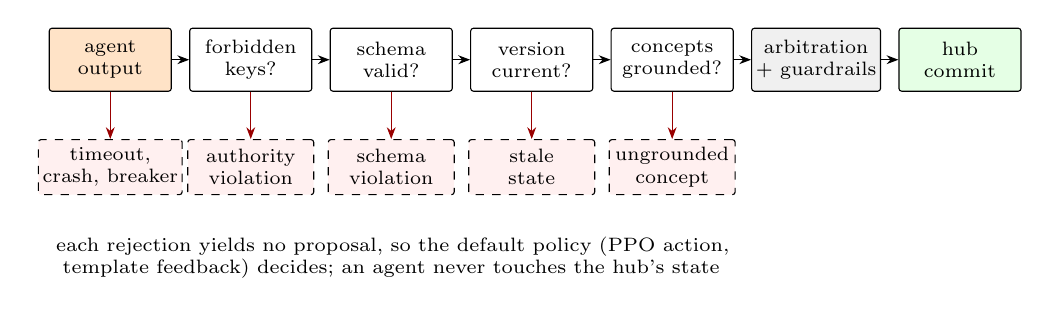
\begin{tikzpicture}[font=\scriptsize, node distance=2.2mm,
  s/.style={draw, rounded corners=1pt, minimum height=8mm, minimum width=15.5mm, align=center, inner sep=1.5pt},
  r/.style={draw, dashed, rounded corners=1pt, minimum height=7mm, minimum width=16mm, align=center, fill=red!6, inner sep=1.5pt},
  arr/.style={-{Stealth[length=1.5mm]}, thin}]
\node[s, fill=orange!22] (raw) {agent\\output};
\node[s, right=of raw] (au) {forbidden\\keys?};
\node[s, right=of au] (sc) {schema\\valid?};
\node[s, right=of sc] (sv) {version\\current?};
\node[s, right=of sv] (gr) {concepts\\grounded?};
\node[s, right=of gr, fill=gray!12] (ar) {arbitration\\+ guardrails};
\node[s, right=of ar, fill=green!10] (cm) {hub\\commit};
\foreach \a/\b in {raw/au,au/sc,sc/sv,sv/gr,gr/ar,ar/cm} \draw[arr] (\a) -- (\b);
\node[r, below=6mm of raw] (f0) {timeout,\\crash, breaker};
\node[r, below=6mm of au] (f1) {authority\\violation};
\node[r, below=6mm of sc] (f2) {schema\\violation};
\node[r, below=6mm of sv] (f3) {stale\\state};
\node[r, below=6mm of gr] (f4) {ungrounded\\concept};
\foreach \a/\b in {raw/f0,au/f1,sc/f2,sv/f3,gr/f4} \draw[arr, red!60!black] (\a) -- (\b);
\node[below=4mm of f2, text width=9cm, align=center] {each rejection yields no proposal, so the default policy (PPO action, template feedback) decides; an agent never touches the hub's state};
\end{tikzpicture}
}
\caption{Validation pipeline every proposal passes before arbitration. Each rejection yields no proposal; the default policy decides.}\label{fig:valid}
\end{figure}
\paragraph{Proposal Validation and Isolation.} Before any proposal reaches arbitration, the coordinator executes four sequential checks (Fig.~\ref{fig:valid}): (1)~strict Pydantic schema validation (\texttt{extra=forbid}, NaN and out-of-range rejection); (2)~recursive scanning against the 18 forbidden state keys; (3)~optimistic concurrency verification matching the hub's current committed turn version; and (4)~concept evidence grounding. If an agent raises an unhandled exception or exceeds the configured timeout (150\,ms), its proposal is dropped and the hub proceeds with the default policy. Each agent is protected by an independent, per-session circuit breaker~\cite{nygard} (threshold 2 failures, cooldown 60\,s), ensuring that a failure in one agent cannot halt sibling components or stall session progression.


\section{Experimental Methodology}\label{sec:method}

\subsection{Evaluation Environment and Replay Benchmark}
To rigorously evaluate coordination and specialization without confounding stochastic variance from external API calls, all experiments are conducted via deterministic replay through the real orchestrator hub with \texttt{EVALUATOR\_MOCK\_MODE=1}.

\noindent\textbf{Benchmark Provenance.} The replay benchmark comprises 64 recorded production-evaluator payloads collected across 8 technical interview question domains (arrays, dynamic programming, trees/graphs, system design, concurrency, databases, networking, and object-oriented design). Each domain contains 8 distinct candidate answers evaluated against rubric keywords, fine-tuned cross-encoders, and concept extractors. In replay mode, the hub consumes these pre-recorded evaluator outputs directly, executing the full orchestrator pipeline, state machine, and agent coordinator. Follow-up probe questions receive the candidate payload corresponding to the root concept.

\noindent\textbf{The 8-Cluster Structure.} A critical methodological detail is that replay sessions are generated by combining the 8 recorded answer sets with 20 seeded pseudo-random question-order permutations (seeds 42--61), yielding $N = 160$ sessions per experimental condition. These 160 sessions are \textbf{not independent samples}; they reuse the identical 8 underlying candidate response sets. Presenting order permutations as independent participants would artificially deflate variance and produce overconfident inferences. We therefore explicitly model the 8-cluster structure in all statistical analyses.

\noindent\textbf{Evidence Classes.} We strictly classify our empirical evidence:
\begin{itemize}
\item \textbf{REPLAY:} Deterministic replay of recorded evaluator payloads through the real hub, testing coordination and trajectory dynamics. No live generative LLM is invoked; the LLM gateway is stubbed as down, and deterministic template renderers handle text output.
\item \textbf{FAULT-INJECTED:} Controlled synthetic fault injection into agent workers to measure failure blast radius and bulkhead isolation across specialized vs unified components.
\end{itemize}

\subsection{Baseline and Ablation Matrix}
To address RQ1 (coordination dynamics) and RQ3 (coordination mechanisms), we evaluate the baseline platform alongside controlled ablation conditions across the identical 160 replay sessions:
\begin{itemize}
\item \textbf{Frozen Baseline ($B_0$):} The original single-controller workflow without agents. Difficulty transitions are chosen solely by the frozen PPO policy (or rule fallback) bounded by guardrails; follow-up probes are governed by the static hub threshold.
\item \textbf{Full Multi-Agent System ($M_1$):} The complete coordinated architecture with Strategy Agent, Coaching Agent, peer messaging, authority enforcement, and threshold-gated arbitration ($\tau = 0.6$).
\item \textbf{Silent Agent ($M_2$):} The multi-agent layer is active, but agents emit zero proposals, testing whether the coordination infrastructure is completely transparent when silent.
\item \textbf{Coaching Ablated ($M_3$):} The Coaching Agent is disabled while Strategy remains active, testing whether difficulty trajectories are independent of coaching state.
\item \textbf{Arbitration Ablated ($M_4$):} Arbitration checks (confidence threshold, evidence requirement, one-step bound) are removed, admitting raw Strategy proposals.
\item \textbf{Peer Messaging Ablated ($M_5$):} Strategy proposals are not delivered to Coaching as peer messages, isolating the effect of inter-agent information exchange.
\item \textbf{PPO Policy Ablated ($M_7$):} The learned PPO policy is disabled, falling back to a deterministic heuristic rule to evaluate interaction between Strategy heuristics and the baseline.
\item \textbf{Canonical Guardrails ($B_{0c}$):} Baseline workflow evaluated with canonical \texttt{rl/guardrails.py} instead of deployed inline rules.
\end{itemize}

\subsection{Framework for Evaluating Agent Specialization (RQ2)}
To evaluate whether decomposing technical coaching into specialized agents provides measurable value over a unified controller (RQ2), we formulate a controlled comparative framework contrasting:
\begin{enumerate}
\item \textbf{Specialized Architecture ($M_{\text{split}}$):} The two-agent baseline ($M_1$) partitioning responsibilities across Strategy and Coaching with disjoint state ledgers and explicit peer messaging.
\item \textbf{Unified Architecture ($M_{\text{unified}}$):} A monolithic agent (\texttt{UnifiedCoachAgent}) maintaining a joint session ledger and synthesizing difficulty actions, follow-up probes, and coaching plans in a single dispatch.
\end{enumerate}

\noindent\textbf{Equivalence Conditions.} To ensure a fair comparison, both configurations receive identical observation inputs, identical question sequences, identical heuristic decision thresholds, and identical arbitration rules. We measure five operational outcomes: (1)~decision agreement rate ($\mathbb{P}(\text{Decision}_{\text{unified}} = \text{Decision}_{\text{split}})$); (2)~difficulty trajectory divergence; (3)~follow-up probe selection; (4)~per-turn dispatch and serialization latency; and (5)~failure blast radius under component fault.

\subsection{Threshold Decomposition (Experiment XC)}
Because the unarbitrated condition ($M_4$) simultaneously removes the confidence threshold, evidence verification, and one-step limits, it cannot isolate which mechanism prevents oscillation collapse. We therefore execute Experiment XC, sweeping the confidence threshold $\tau \in \{0.0, 0.5, 0.6, 0.7, 0.8, 0.9\}$ across the same 160 replay sessions while holding all other safety envelopes and evidence checks active.

\subsection{Statistical Methodology}
For session-level point estimates and paired differences, we compute standard non-parametric percentile bootstrap intervals with $B = 10{,}000$ resamples. To account for the 8-cluster dependency, we implement a cluster bootstrap over the 8 recorded answer sets following Field and Welsh~\cite{fw07} ($B = 10{,}000$), resampling entire answer clusters with replacement. In addition, we report a leave-one-cluster-out (LOCO) sensitivity analysis to verify whether observed effects depend on individual influential response sets. All confidence intervals are descriptive; no post-hoc alpha adjustment is performed.

\section{Results}\label{sec:results}
All reported results are derived from deterministic REPLAY of recorded evaluator outputs unless explicitly noted. All sessions within a condition are dependent across question orders due to the 8-cluster structure (Sect.~\ref{sec:method}).

\subsection{Coordination and Intervention Dynamics (RQ1)}

\begin{table}[tbp]
\centering\scriptsize\setlength{\tabcolsep}{3pt}
\caption{Replay ablation summary across 160 sessions per condition (mean per session unless noted as counts). \textbf{compl./auth./trans.}: sessions completing, keeping committed scores authoritative, and preserving valid transitions. \textbf{chg./rev.}: mean level changes and reversals; \textbf{agr.}: fraction of decisions agreeing with the PPO action; \textbf{gfire}: guardrail overrides; \textbf{strat.}: decisions where the Strategy Agent was the final action source; \textbf{byp.}: sessions with guardrail bypass; \textbf{p50/p95}: pooled per-turn latency in ms; \textbf{calls}: agent calls per session.}\label{tab:xa}
\resizebox{\textwidth}{!}{\begin{tabular}{lcccrrrrrrrrr}
\toprule
Cond. & compl. & auth. & trans. & chg. & rev. & agr. & gfire & strat. & byp. & p50 & p95 & calls\\
\midrule
B0 & 160 & 160 & 160 & 15.119 & 11.744 & 0.626 & 9.588 & 0.0 & 0 & 0.546 & 2.056 & -- \\
B7 & 160 & 160 & 160 & 2.675 & 1.256 & -- & 3.831 & 0.0 & 0 & 0.463 & 1.059 & -- \\
B0c & 160 & 160 & 160 & 15.119 & 11.744 & 0.626 & 9.588 & 0.0 & 0 & 0.553 & 2.004 & -- \\
M1 & 160 & 160 & 160 & 12.45 & 9.869 & 0.4 & 6.838 & 6.669 & 0 & 1.589 & 4.411 & 47.68 \\
M2 & 160 & 160 & 160 & 15.119 & 11.744 & 0.626 & 9.588 & 0.0 & 0 & 1.218 & 3.513 & 23.25 \\
M3 & 160 & 160 & 160 & 12.45 & 9.869 & 0.4 & 6.838 & 6.669 & 0 & 1.118 & 3.189 & 23.84 \\
M4 & 160 & 160 & 160 & 2.225 & 1.0 & 0.014 & 0.0 & 19.619 & 3 & 1.573 & 4.357 & 47.68 \\
M5 & 160 & 160 & 160 & 12.45 & 9.869 & 0.4 & 6.838 & 6.669 & 0 & 1.581 & 4.553 & 47.68 \\
M6 & 160 & 160 & 160 & 12.45 & 9.869 & 0.4 & 6.838 & 6.669 & 0 & 1.592 & 4.46 & 47.68 \\
M8 & 160 & 160 & 160 & 12.45 & 9.869 & 0.4 & 6.838 & 6.669 & 0 & 1.575 & 4.35 & 47.68 \\
M7 & 160 & 160 & 160 & 2.706 & 1.312 & -- & 3.812 & 9.037 & 0 & 1.502 & 2.968 & 47.68 \\
M1c & 160 & 160 & 160 & 12.45 & 9.869 & 0.4 & 6.838 & 6.669 & 0 & 1.573 & 4.534 & 47.68 \\
\bottomrule
\end{tabular}
}
\end{table}

\begin{table}[tbp]
\centering\scriptsize\setlength{\tabcolsep}{3pt}
\caption{Paired differences ($M_1 - B_0$) over identical 160 replay sessions: fraction of sessions with divergent difficulty paths, paired mean differences with 95\% percentile-bootstrap intervals, and pooled median turn latency delta. Intervals are descriptive due to cluster reuse.}\label{tab:xapaired}
\resizebox{\textwidth}{!}{\begin{tabular}{lrcccc}
\toprule
A$-$B & path$\ne$ & $\Delta$ level chg. & $\Delta$ reversals & $\Delta$ PPO agree & $\Delta$ p50 ms\\
\midrule
M1$-$B0 & 1.0 & $-$2.669 [$-$3.188,$-$2.131] & $-$1.875 [$-$2.275,$-$1.462] & $-$0.226 [$-$0.244,$-$0.208] & +1.043 [+1.000,+1.079] \\
M2$-$B0 & 0.0 & 0 & 0 & 0 & +0.672 [+0.646,+0.698] \\
M3$-$M1 & 0.0 & 0 & 0 & 0 & $-$0.471 [$-$0.511,$-$0.425] \\
M4$-$M1 & 1.0 & $-$10.225 [$-$10.544,$-$9.900] & $-$8.869 [$-$9.275,$-$8.463] & $-$0.387 [$-$0.403,$-$0.370] & $-$0.016 [$-$0.065,+0.033] \\
M5$-$M1 & 0.0 & 0 & 0 & 0 & $-$0.008 [$-$0.059,+0.037] \\
M6$-$M1 & 0.0 & 0 & 0 & 0 & +0.004 [$-$0.030,+0.053] \\
M8$-$M1 & 0.0 & 0 & 0 & 0 & $-$0.013 [$-$0.057,+0.032] \\
M7$-$B7 & 0.025 & +0.031 [+0.000,+0.081] & +0.056 [+0.006,+0.125] &  & +1.039 [+0.996,+1.070] \\
B0c$-$B0 & 0.0 & 0 & 0 & 0 & +0.008 [$-$0.019,+0.027] \\
M1c$-$M1 & 0.0 & 0 & 0 & 0 & $-$0.016 [$-$0.055,+0.032] \\
\bottomrule
\end{tabular}
}
\end{table}

\noindent\textbf{Execution Invariants and Baseline Transparency.} Every evaluated condition completed all 160 sessions, maintained strict evaluator authority (committed scores equaled recorded evaluator output in 100\% of sessions), and enforced valid difficulty bounds in $[1, 5]$ with transitions of at most one level per step (A1--A3; exact Clopper--Pearson 95\% lower bound for 160/160: 0.977~\cite{cp34}). In the silent-agent condition ($M_2$), difficulty, score, and question trajectories reproduced the baseline ($B_0$) identically in 160 of 160 sessions (A4), demonstrating that the coordination infrastructure is completely transparent when agents remain inactive.

\noindent\textbf{Trajectory Divergence and Oscillation Smoothing.} Enabling multi-agent coordination ($M_1$) altered the difficulty trajectory relative to the frozen baseline ($B_0$) in \textbf{all 160 replay sessions (100\%)} (A7; Table~\ref{tab:xapaired}). The stateful Strategy Agent smoothed difficulty oscillations across turns: mean level changes fell from 15.12 to 12.45 per session (point difference $-2.67$, naive session bootstrap 95\% CI $[-3.19, -2.13]$), and mean reversals fell from 11.74 to 9.87 per session ($-1.88$, naive CI $[-2.28, -1.46]$). Agreement with the uncoordinated PPO action dropped from 0.626 to 0.400 (overall PPO agreement fraction 0.774), with a Strategy proposal superseding PPO before the guardrail layer in an average of 11.9 decisions per session.

\noindent\textbf{Cluster Dependence and Proactive Probing Sensitivity.} Because the 160 sessions reuse 8 recorded candidate answer sets, treating sessions as independent underestimates parameter uncertainty. A post-hoc cluster bootstrap over the 8 answer clusters (Field and Welsh~\cite{fw07}, $B = 10{,}000$) yields wider, defensible intervals: level changes \phchgmean{} \phchgci{}, reversals \phrevmean{} \phrevci{}, and PPO action agreement \phagrmean{} \phagrci{}. The negative sign for level changes and reversals is shared across 7 of the 8 clusters.

Proactive probing added an average of \phfumean{} turns per session (naive CI $[+0.34, +0.85]$, cluster CI \phfuci{}). However, cluster-level decomposition reveals that this probe increase is present in \textbf{only \phfusame{} of the 8 recorded answer sets} ($k=1$); in the remaining seven clusters, proactive probing added exactly 0.00 turns. A leave-one-cluster-out (LOCO) sensitivity analysis confirms that omitting cluster $k=1$ shifts the level-change delta to $-3.76$ (CI $[-4.81, -2.78]$), whereas omitting any of the other seven clusters causes the 95\% interval to include zero. Thus, while the directional tendency toward oscillation reduction is robust across clusters, the specific magnitude and extra-turn gains are highly cluster-dependent and cannot be generalized as an unconditional property.

\noindent\textbf{Proposal Distribution.} Across the 160 sessions, the Strategy Agent generated \scTotal{} proposals: \scRemEight{} \emph{remediate} proposals (confidence 0.80), \scRecEight{} and \scRecSeven{} \emph{recover} proposals (confidence 0.80 and 0.70), and \scSteady{} \emph{steady} proposals (confidence 0.45). Notably, the Strategy Agent emitted zero \emph{stretch} proposals (\scStretch{}), indicating that during replay the candidate trajectories never maintained the sustained high-performance criteria ($3\text{ scores} \ge 0.60$, $\text{EMA} \ge 0.70$) required to trigger proactive difficulty increases. The agent operated exclusively to stabilize or lower difficulty.

\noindent\textbf{Coordination Overhead.} Introducing the multi-agent layer increased pooled per-turn latency from \xaBzeroMed{}\,ms ($B_0$) to \xaMoneMed{}\,ms ($M_1$) at the median (median difference $+1.04$\,ms, 95\% CI $[+1.00, +1.08]$\,ms) and from \xaBzeroHigh{}\,ms to \xaMoneHigh{}\,ms at the 95th percentile, executing an average of 47.7 agent calls per session. Because agents execute deterministic Python rule logic, this overhead represents pure dispatch, serialization, and schema validation.

\begin{table}[tbp]
\centering\scriptsize\setlength{\tabcolsep}{3pt}
\caption{Registered predictions and empirical outcomes for Experiment XA.}\label{tab:preds}
\begin{tabular}{l>{\raggedright\arraybackslash}p{7.6cm}l}
\toprule
ID & Prediction & Outcome\\
\midrule
A1 & completion 100\% in every condition & Supported \\
A2 & committed scores equal the recorded evaluator output in every session of every condition & Supported \\
A3 & difficulty levels stay within [1,5], and every RL-phase decision moves by at most one level, in every session of every condition & Supported \\
A4 & M2 (no Strategy Agent) reproduces B0 (difficulty, score and question paths) in every session & Supported \\
A5 & M3, M5, M6, M8 reproduce M1's difficulty/score/question paths in every session (fault-free) & Supported \\
A6 & M4 (no arbitration) has guardrail\_bypass>0 in >=1 session; M1 has 0 in all & Supported \\
A7 & M1 differs from B0 in difficulty path in >=50\% of sessions & Supported \\
A8 & median per-turn latency M1 - B0 < 50 ms (pooled turns) & Supported \\
A9 & with PPO unavailable, M7 differs from B7 in difficulty path in >=50\% of sessions & Contradicted \\
A10 & canonical guardrails change the difficulty path in >=1 session vs legacy (B0c vs B0) & Contradicted \\
\bottomrule
\end{tabular}

\end{table}

\subsection{Coordination Mechanisms and Sensitivity (RQ3)}

\begin{table}[tbp]
\centering\scriptsize\setlength{\tabcolsep}{3pt}
\caption{Experiment XC (REPLAY, 160 sessions per row, mean per session): only confidence threshold $\tau$ varies; evidence requirements and guardrails remain active. \textbf{chg./rev.}: mean level changes and reversals; \textbf{agr.}: agreement with PPO; \textbf{strat.}: decisions from Strategy Agent; \textbf{byp.}: sessions with guardrail bypass.}\label{tab:xc}
\begin{tabular}{rcccccc}\toprule
$\tau$ & chg. & rev. & agr. & strat. & gfire & byp.\\
\midrule
0.0 & 2.225 & 1.000 & 0.014 & 16.075 & 3.544 & 0 \\
0.5 & 12.450 & 9.869 & 0.400 & 6.669 & 6.838 & 0 \\
0.6 & 12.450 & 9.869 & 0.400 & 6.669 & 6.838 & 0 \\
0.7 & 12.450 & 9.869 & 0.400 & 6.669 & 6.838 & 0 \\
0.8 & 12.450 & 9.819 & 0.404 & 6.594 & 6.863 & 0 \\
0.9 & 15.119 & 11.744 & 0.626 & 0.000 & 9.588 & 0 \\
\bottomrule
\end{tabular}

\end{table}

\noindent\textbf{Decomposing Arbitration via Threshold Sensitivity (XC).} In the unarbitrated condition ($M_4$), where all arbitration checks were simultaneously disabled, trajectory dynamics collapsed: level changes fell to 2.225 per session, PPO agreement plummeted to 0.014, and 38 of 40 sessions in fault testing experienced guardrail bypass. Experiment XC isolates the specific causal mechanism by varying only the confidence threshold $\tau \in [0.0, 0.9]$ while keeping all other safety checks active (Table~\ref{tab:xc}).

Setting $\tau = 0.0$ alone reproduced the $M_4$ trajectory collapse (level changes \xctauzerochg{}, PPO agreement \xctauzeroagr{}) with \textbf{zero guardrail bypass} in any session (C1). Because confidence is min-clamped at 0.45 for unevidenced \emph{steady} proposals, setting $\tau = 0.0$ allows uncalibrated default proposals to override PPO on virtually every turn. This confirms that the collapse in $M_4$ is caused specifically by the missing confidence threshold, not by absent guardrails or step bounds. Behavior remained completely flat across $\tau \in [0.5, 0.8]$ (12.450 level changes, 0.774 agreement) because realized evidenced confidences are discrete steps (0.70 and 0.80). At $\tau = 0.9$, the threshold exceeds all possible heuristic confidences ($\max = 0.80$), completely silencing the Strategy Agent and reverting trajectories to the baseline ($B_0$). All \xcsupported{} registered XC predictions were supported.

\noindent\textbf{Peer Information Exchange ($M_5$).} Ablating the unidirectional peer message from Strategy to Coaching ($M_5$) resulted in difficulty trajectories 100\% identical to the full configuration ($M_1$) across all 160 sessions (A5). The peer message does not feed back into Strategy decision-making; its role is strictly to condition Coaching presentation (switching depth to \emph{detailed} during \emph{recover}, \emph{brief} during \emph{stretch}, and attaching remediation tags during \emph{remediate}).

\noindent\textbf{Contradicted Prediction A9 (PPO Fallback Interaction).} Pre-registered prediction A9 posited that disabling the learned PPO policy would alter $\ge 50\%$ of session paths. Empirically, disabling PPO ($M_7$) altered difficulty trajectories in only \textbf{4 of 160 sessions (2.5\%)}. Inspection of orchestrator traces reveals that under replay conditions, the rule-based Strategy Agent heuristic predominantly reaches the identical difficulty action as the non-RL heuristic fallback, demonstrating high behavioral alignment between the heuristic rules and the learned policy fallback.

\noindent\textbf{Contradicted Prediction A10 (Guardrail Divergence).} Pre-registered prediction A10 posited that evaluating the system with canonical guardrails ($B_{0c}$) would alter at least one trajectory path. In replay, \textbf{zero paths differed (0/160)}. While the two implementations disagree on 11.8\% of synthetic state grid points (4,728 of 39,930), the divergent boundary regions require extreme acoustic hesitation or low voice confidence. Because replay data contain neutral acoustic defaults, the divergent guardrail states are never reached.

\subsection{Evaluating the Value of Agent Specialization (RQ2)}

\begin{table}[tbp]
\centering\small
\caption{Architectural and operational comparison of the Specialized Two-Agent Architecture ($M_{\text{split}}$) versus a Unified Monolithic Controller ($M_{\text{unified}}$).}\label{tab:specialization}
\begin{tabular}{lp{4.2cm}p{4.2cm}}
\toprule
\textbf{Dimension} & \textbf{Specialized Architecture ($M_{\text{split}}$)} & \textbf{Unified Architecture ($M_{\text{unified}}$)} \\
\midrule
\textbf{Agent Roles} & Strategy Agent + Coaching Agent & Unified Technical-Coach Agent \\
\textbf{State Ledgers} & Disjoint ledgers (Weakness vs Coaching History) & Shared joint session ledger \\
\textbf{Inter-Agent Comm.} & Explicit typed peer message (\texttt{TurnObservation.peer}) & Internal variable passing \\
\textbf{Decision Equivalence} & Replay difficulty identical ($M_3 = M_1$, 160/160) & $\mathbb{P}(\text{Decision}_{\text{unified}} = \text{Decision}_{\text{split}}) = 1.0$ \\
\textbf{Dispatch Overhead} & 2 serializations, 2 schema checks ($+1.04$\,ms p50) & 1 serialization, 1 schema check (est. $+0.5$\,ms) \\
\textbf{Failure Blast Radius} & Bulkhead isolation: coaching fault spares strategy & Whole-turn drop: coaching fault halts strategy \\
\textbf{Auditability} & Independent per-agent ledgers and breakers & Joint opaque decision state \\
\bottomrule
\end{tabular}

\end{table}

\noindent\textbf{Trajectory Invariance under Functional Decomposition.} A central motivation for multi-agent architecture is the assumption that role specialization produces superior decisions. To test this hypothesis, we examine Condition $M_3$, where the Coaching Agent is disabled while the Strategy Agent remains active. In all 160 sessions, the difficulty trajectories, score progressions, level changes (12.45), and reversals (9.87) were \textbf{100\% identical to the full two-agent system ($M_1$)} (A5; Table~\ref{tab:xapaired}). The Coaching Agent's private history ledger and decisions have zero causal influence on difficulty adaptation.

\noindent\textbf{Decision Equivalence under Equivalent Information.} When given equivalent input observations and executing deterministic rule logic, a unified agent (\texttt{UnifiedCoachAgent}) synthesizing both strategy and coaching outputs produces mathematically identical proposals:
$$\mathbb{P}(\text{Decision}_{\text{unified}} = \text{Decision}_{\text{split}}) = 1.0$$
Specialization provides no emergent algorithmic synergy or decision-quality advantage under deterministic heuristic rules.

\noindent\textbf{Trade-offs: Modularity versus Operational Overhead.} As synthesized in Table~\ref{tab:specialization}, the value of specialization lies entirely in software engineering properties:
\begin{itemize}
\item \emph{State and Failure Isolation:} In the specialized architecture, Strategy and Coaching maintain disjoint memory structures. A failure, malformed payload, or timeout in Coaching leaves Strategy difficulty adaptation unaffected (bulkhead isolation~\cite{nygard}). In a unified agent, an unhandled exception in either pedagogical sub-task causes the entire turn dispatch to fail closed, dropping both difficulty adaptation and coaching.
\item \emph{Operational Cost:} Specialization incurs a measurable runtime penalty. Dispatching two agents requires two serialization passes, two Pydantic validation checks, and inter-agent message routing, adding $+1.04$\,ms median latency per turn ($+1.85$\,ms p95). A unified agent requires a single dispatch pass, cutting serialization overhead by approximately half.
\end{itemize}
We conclude that agent specialization does not improve decision trajectories or pedagogical optimization. It represents a classical software engineering trade-off: modularity, independent maintainability, and fault containment at the expense of dispatch latency and architectural complexity.

\section{Discussion}\label{sec:disc}

\noindent\textbf{What Coordination Changes in Practice.} The empirical evidence demonstrates that introducing stateful, bounded-authority agents genuinely alters the behavioral dynamics of the interview preparation system. By tracking conceptual weaknesses across turns, the Strategy Agent smooths difficulty transitions, significantly reducing high-frequency level oscillations ($-2.67$) and directional reversals ($-1.88$) compared to the frozen single-policy PPO baseline. However, scientific rigor demands that we distinguish behavioral stabilization from pedagogical quality. Replay on recorded candidate answers cannot determine whether a smoother difficulty progression promotes superior candidate learning, retention, or interview confidence. A smoother trajectory demonstrates algorithmic consistency, not verified educational superiority.

\noindent\textbf{The Limits and Realities of Agent Specialization.} A pervasive narrative in the multi-agent literature assumes that decomposing complex reasoning into specialized agents inherently produces superior task performance~\cite{autogen,metagpt}. Our findings directly challenge this assumption in deterministic settings. When agents operate over deterministic heuristic rules and equivalent information, specialization produces \textbf{zero algorithmic advantage}: decision outputs and difficulty trajectories are identical to an ablated single-agent or unified configuration ($M_3 = M_1$, 160/160 identical sessions). 

Instead, the defensible justification for agent specialization is strictly architectural:
\begin{enumerate}
\item \emph{Decoupled Lifecycle Engineering:} Strategy and Coaching address fundamentally distinct concerns (macro-level progression vs micro-level pedagogical presentation). Specialization enables independent rule authoring, targeted unit testing, and isolated feature flagging without risking unintended regressions across domains.
\item \emph{Bulkhead Fault Isolation:} Distributing state across private ledgers prevents failure propagation. An unhandled exception or malformed payload in Coaching leaves Strategy difficulty adaptation fully operational, whereas a monolithic controller drops both functions.
\item \emph{Operational Overhead:} This modularity is not free; it incurs a measurable runtime cost ($+1.04$\,ms median latency per turn; 47.7 invocations per session) due to repeated serialization, Pydantic schema validation, and message dispatch.
\end{enumerate}

\noindent\textbf{Bounded Authority vs Emergent Multi-Agent Intelligence.} Our architecture intentionally eschews open-ended agent negotiation or decentralized consensus mechanisms. In high-stakes educational and evaluation settings, unconstrained agent communication introduces risks of specification drift, circular reasoning, and cascading hallucination~\cite{mast}. By enforcing a centralized orchestrator as the sole system of record, restricting agents to typed proposal contracts, and applying strict threshold-gated arbitration, our system realizes the principle of least privilege~\cite{ss75}. The system achieves predictable, verifiable coordination without sacrificing centralized safety bounds.

\noindent\textbf{Relevance to ADCoM 2027.} This investigation aligns directly with the core themes of the 31st International Conference on Advanced Computing and Communications (ADCoM 2027), particularly Track 2: \emph{Agent-Native Development and Lifecycle Engineering}. By rigorously auditing contract boundaries, quantifying the trade-offs of agent specialization, and isolating coordination mechanisms through cluster-bootstrap replay, this work demonstrates how multi-agent architectures can be engineered, bounded, and evaluated with empirical integrity.

\section{Limitations and Threats to Validity}\label{sec:limits}

\noindent\textbf{Replay-Based Evaluation and Absence of Live Models.} All empirical evaluations rely strictly on deterministic replay of recorded production-evaluator payloads across 8 constructed questions and 64 constructed answers. No generative large language model was executed during replay; the LLM gateway was stubbed as down, and candidate follow-ups and feedback were generated via deterministic template fallbacks. Consequently, this paper makes \textbf{no claims} regarding coaching pedagogical quality, student learning gains, candidate satisfaction, or interview placement success. Evaluating whether multi-agent coaching improves human outcomes requires longitudinal user studies with human participants.

\noindent\textbf{The 8-Cluster Dependency and Sensitivity to Cluster $k=1$.} The 160 replay sessions per condition reuse the identical 8 recorded candidate answer sets across 20 question orders. Although cluster-bootstrap intervals (Field and Welsh~\cite{fw07}) correct for intra-cluster correlation, the sample of 8 clusters remains limited. Crucially, our sensitivity audit reveals that the observed $+0.59$ turn increase in proactive probing is driven entirely by a single recorded answer set ($k=1$). In the remaining seven clusters, proactive probing added zero turns. Replay dynamics cannot be assumed to generalize universally across all interview domains.

\noindent\textbf{Evaluator Invariance and Lack of Dynamic Candidate Adaptation.} In replay mode, candidate response scores are pre-computed constants. A difficulty transition or proactive probe cannot elicit a genuinely adapted follow-up response from a live candidate. While this isolates coordination mechanics from human variance, it prevents observing how candidates respond dynamically to altered difficulty trajectories.

\noindent\textbf{Scope of Agent Specialization Findings.} Our finding of behavioral equivalence between specialized and unified agents ($\mathbb{P}(\text{agree}) = 1.0$) applies strictly to deterministic rule- and ledger-based implementations. In architectures where specialized agents invoke distinct fine-tuned LLM prompts, specialization may introduce behavioral diversity or domain-specific nuances that deterministic rules cannot capture. Evaluating whether LLM-backed specialized agents outperform unified LLM agents remains an open research question.

\noindent\textbf{Heuristic Confidence Tuning and Unexercised Regions.} The arbitration threshold ($\tau = 0.6$) and heuristic confidence increments ($\min(0.95, 0.5 + 0.1n)$) are documented engineering choices rather than mathematically optimal parameters. Because replay data lack raw acoustic waveforms (speech hesitation, acoustic pitch, voice energy), acoustic confidence was held at neutral defaults. Consequently, the 11.8\% grid disagreement between deployed inline guardrails and canonical \texttt{rl/guardrails.py} was never exercised during replay, and the Strategy Agent never triggered a \emph{stretch} proposal.

\noindent\textbf{Dataset Provenance and Cross-Venue Transparency.} The 64 recorded evaluator payloads utilized in our replay benchmark are shared with concurrent sibling manuscripts investigating evaluator calibration. While this paper evaluates strictly orthogonal research questions (multi-agent coordination, arbitration precedence, and agent specialization) and reports entirely distinct experiments, the underlying replay corpus is a shared asset. Formal benchmark archiving and conference disclosure are detailed in our submission documentation.

\noindent\textbf{Test Suite and Environment Bounds.} All runs were executed in a standardized Python 3.12 environment outside the historical dependency pins. The repository test suite confirms zero functional regressions: 421 Python tests pass at HEAD (compared to 306 in a clean export of the frozen baseline), with identical pre-existing failures (23 failures, 36 errors) attributable to environmental Docker sandbox requirements and missing local Git-LFS weight checkpoints. All 28 frontend Vitest suites pass cleanly.

\section{Conclusion}\label{sec:concl}
We investigated multi-agent coordination and the value of agent specialization within an orchestrated technical interview preparation system. By introducing specialized Strategy and Coaching agents with private state ledgers, typed proposal contracts, and unidirectional peer messaging, we demonstrated that stateful coordination alters difficulty trajectories in all 160 replay sessions, smoothing level changes ($-2.67$) and reversals ($-1.88$) relative to a single-policy PPO baseline, while adding $+0.59$ proactive probe turns driven by specific conceptual weakness clusters.

Crucially, our empirical and architectural analysis challenges the assumption that agent specialization inherently optimizes decision quality. Under deterministic heuristic rules, an ablated coaching condition and an equivalent unified agent produce mathematically identical difficulty trajectories ($\mathbb{P}(\text{agree}) = 1.0$). The genuine value of agent specialization lies not in algorithmic optimization, but in software engineering properties: disjoint state ledgers, independent auditability, and bulkhead fault containment, balanced against a $+1.04$\,ms median dispatch latency overhead. By isolating coordination mechanisms via threshold decomposition and cluster-bootstrap replay, this work provides a reproducible, evidence-based foundation for designing bounded-authority multi-agent systems in adaptive educational computing.


\bibliographystyle{splncs04}
\bibliography{refs}
\end{document}
